\documentclass{aleph-revista}

\usepackage{tikz}           
\usepackage{aleph-comandos} 
\usepackage{multicol}    
\usepackage{indentfirst}
% \usepackage{natbib}
% \bibliographystyle{abbrvnat}   
\graphicspath{{figures/}}
% \addbibresource{bibliografia.bib}

\titulo{Exercício Computacional 01}
\tituloingles{Método das Diferenças Finitas}

\autor{%
  Natanael Magalhães Cardoso\textsuperscript{1 \faEnvelopeO}
}

\institucion{
\textsuperscript{1}%
  n$^{o}$ USP: 8914122
}

\correo{natanael.mc@usp.br}

\fecha{12 de julho de 2021}

\abstract{
  Este relatório mostra uma solução computacional de um problema do eletromagnetismo com um algorítmo de diferenciação numérica, o Método das Diferenças Finitas. Aqui são expostos dois problemas onde as equipotenciais, as linhas de campo elétrico e o valor da resistência são calculados.
}

\begin{document}
\membrete

\vspace{1em}

\section{Metodologia}

\subsection{Descrição do Programa}

A implementação do programa segue o paradígma de programação funcional. Isto é, o algorítmo é composto por funções puras que dependem apenas de seus parâmetros de entrada e não causam efeitos colaterais no estado do programa. Isto facilita a depuração do programa pela inspeção de cada função separadamente. Já que cada função faz apenas uma tarefa.

A lista a seguir mostra as três funções principais do programa, bem como seus parâmetros de entrada e seus retornos.

\begin{enumerate}
  \item \texttt{template1(k, initial\_value)} $\mapsto$ \texttt{(T)}\\ \texttt{template2(k, initial\_value)} $\mapsto$ \texttt{(T)} \hfill \\
        Estas funções recebem um parâmtro \texttt{k}, que é a constante de escalonamento da matriz. Todas as dimensões da matriz são multiplicadas por esta constante. Quanto maior o valor de \texttt{k}, maior a matriz e menor o tamanho do lado da malha de discretização. O lado $h$ da malha de discretização vale $h=1/k$. O parâmetro \texttt{initial\_value} é o valor inicial de potencial. Esta função retorna uma matriz \texttt{T} a geometria e o estado inicial do problema. Locais preenchidos com vácuo são representados por indeterminação e são despresados no cálculo das funções seguintes.
  \item \texttt{compute\_potential(template, axis, epochs, callbacks)} $\mapsto$ \texttt{(potential, history)} \hfill \\
        Esta função recebe, na ordem de apresentação, um modelo, que é uma matriz que representa a estrutura do problema; o eixo de propagação; a quantidades de épocas, ou iterações, do algorítmo e uma lista de \texttt{callbacks}, que são funções que são executadas durante o processo de convergência. Ela uma tupla contendo a matriz de potencial e o histórico de erro, contendo o valor do erro para cada época.
  \item \texttt{compute\_ef(potential, h)} $\mapsto$ \texttt{(Ex, Ey)} \hfill \\
        Esta função recebe a matriz de potencial, calculada por \texttt{compute\_potential}, e a altura \texttt{h} de cada célula e retorna uma tupla de matrizes \texttt{(Ex, Ey)}, que correspondem às componentes horizontais e verticais do campo elétrico, respectivamente.
  \item \texttt{compute\_resistence(V, l, h, condutivity, Ex, Ey, axis)} $\mapsto$ \texttt{resistence} \hfill \\
        Esta função recebe, na ordem de apresentação, uma diferença de potencial \texttt{V}; o valor da espessura da placa \texttt{l}; o comprimento \texttt{h} de cada célula da malha de discretização; o valor da condutância; os potenciais \texttt{Ex} e \texttt{Ey} calculados pela função \texttt{compute\_ef} e o eixo de propagação. Ela retorna um vetor do comprimento (ou largura) da placa com as resistências calculadas considerando cada linha (ou coluna) de \texttt{Ey} (ou \texttt{Ex}). O valor considerado depende do eixo de propagação.
\end{enumerate}

Para calcular a resistência do problema, as funções são chamadas na ordem mostrada. As funções de vizualização não foram descritas mas estão disponíveis no código-fonte.



\subsection{Inspeção da matriz inicial de potencial}

\begin{figure}[!h]
  \centering
  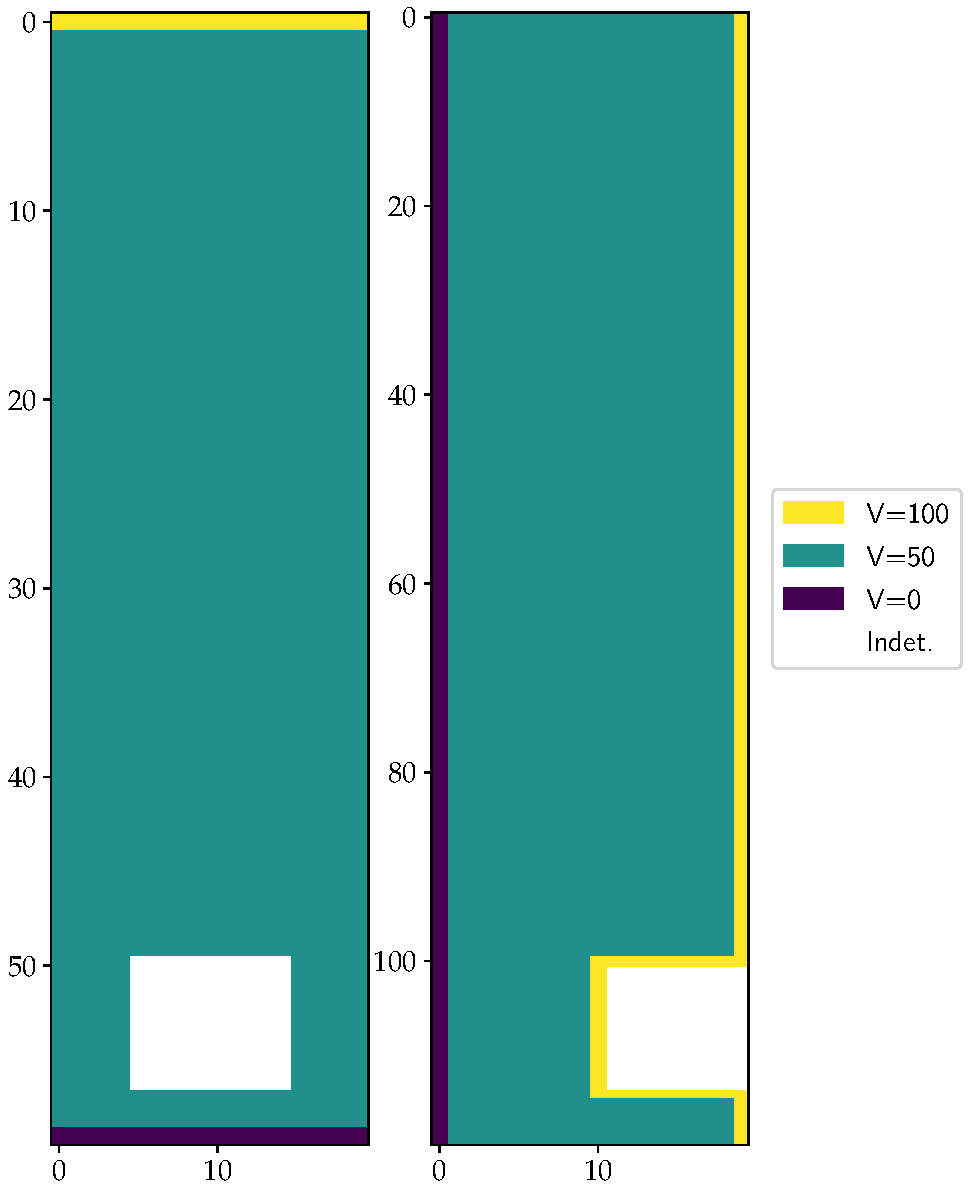
\includegraphics[width=0.6\textwidth]{template}
  \caption{Mapa de cor das matrizes geradas pelas funções \texttt{template1} (esquerda) e \texttt{template2} (direita).}
  \label{fig:template}
\end{figure}

O passo preliminar é a criação da matriz de potencial com os valores iniciais.  A Figura \ref{fig:template} mostra dois gráficos criados para vizualizar a matriz gerada pelas funções \texttt{tamplete1} e \texttt{template2}. Este gráfico mapeia cada valor da matriz para uma cor específica. Esta análise foi feita para verificar se a matriz com os valores iniciais de potencial representa a geometria do problema corretamente. Por motivo de vizualização, foi usado um valor de $k=0.5$ e $k=1$ para os gráficos da esquerda e da direita, respectivamente. Ou seja, cada unidade do gráfico da esquerda representa 2mm da geometria real, enquanto que cada unidade do gráfico da direita representa 1mm da geometria do problema.


Notamos que existem quatro valores (representados pelas cores) distintos nas matrizes, representando os potenciais iniciais em volts, são eles 100, 50, 0 e indeterminado. Os valores 100V e 0V representam os potenciais dos eletrodos e o potenicial 50V, que é o valor médio da DDP entre os eletrodos, é usado como valor inicial. Já o vácuo é representado por uma indeterminação e é mostrado na parte branca do gráfico.

Visto que as matrizes iniciais de potencial são coerentes com as geometrias dos problemas, é possível iniciar o algorítmo de diferenças finitas a partir delas. Os resultados gerados por este algorítmo são mostrados a seguir.

\section{Resultados, Discussão e Conclusão}

\subsection{Equipotenciais}

A Figura \ref{fig:pot} mostra as equipotenciais para ambos os problemas, com $\Delta \varphi = 2V$ no gráfico da esquerda e $\Delta \varphi = 4V$ no gráfico da direita. Ambos com $k=1$ (malha de discretização de 1mm), por motivos de vizualização.

\begin{figure}[!ht]
  \centering
  \begin{tabular}{cc}
    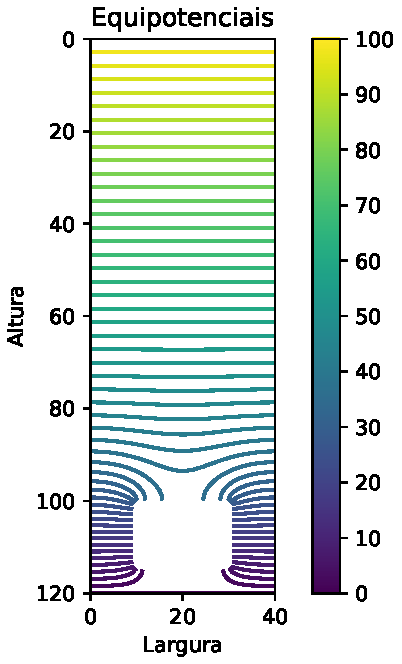
\includegraphics[height=125mm]{p1_equipotenciais} &
    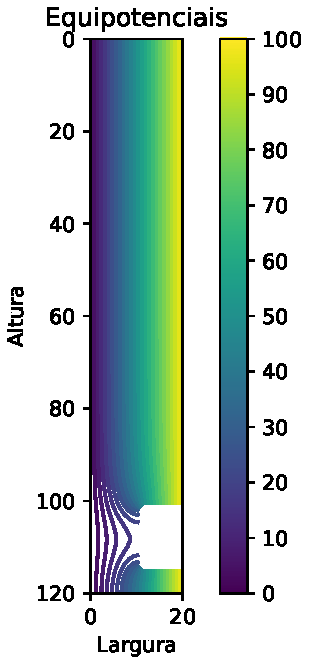
\includegraphics[height=125mm]{p2_equipotenciais}
  \end{tabular}
  \caption{Equipotenciais para o Problema 1 (esquerda) e Problema 2 (direita).}
  \label{fig:pot}
\end{figure}


\newpage
\subsection{Linhas de Campo}

A Figura \ref{fig:campo} mostra as linhas do campo elétrico calculadas nas mesmas condições das equipotenciais (malha de discretização de 1mm), também por motivo de vizualização.

\begin{figure}[!ht]
  \centering
  \begin{tabular}{cc}
    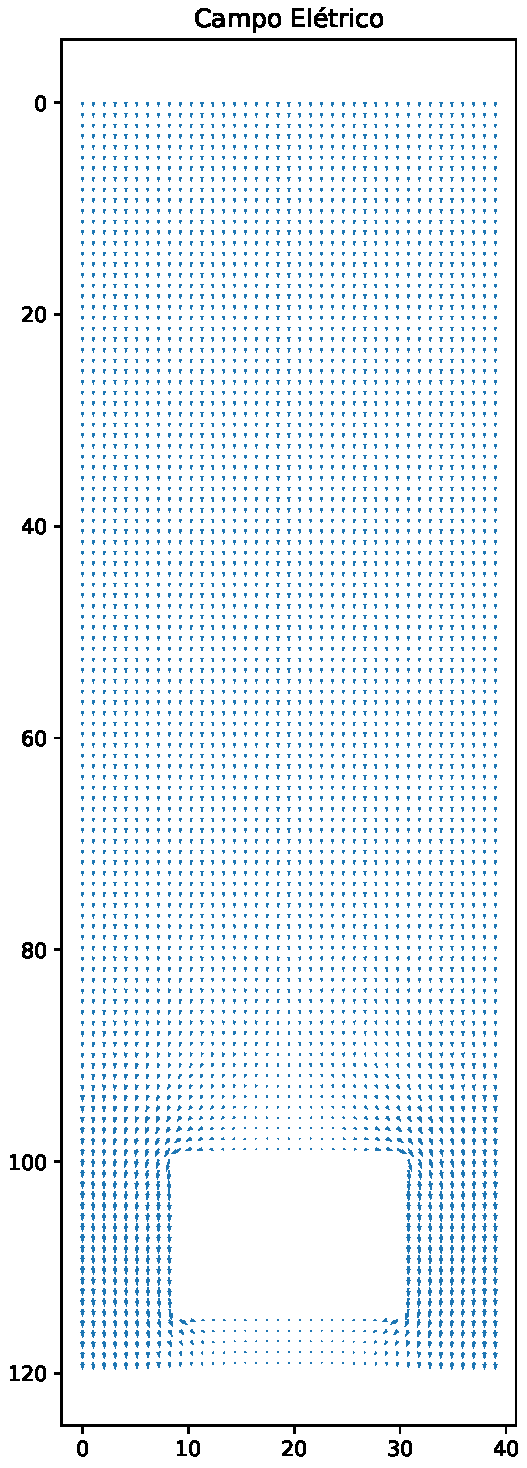
\includegraphics[height=210mm]{p1_campo_eletrico} &
    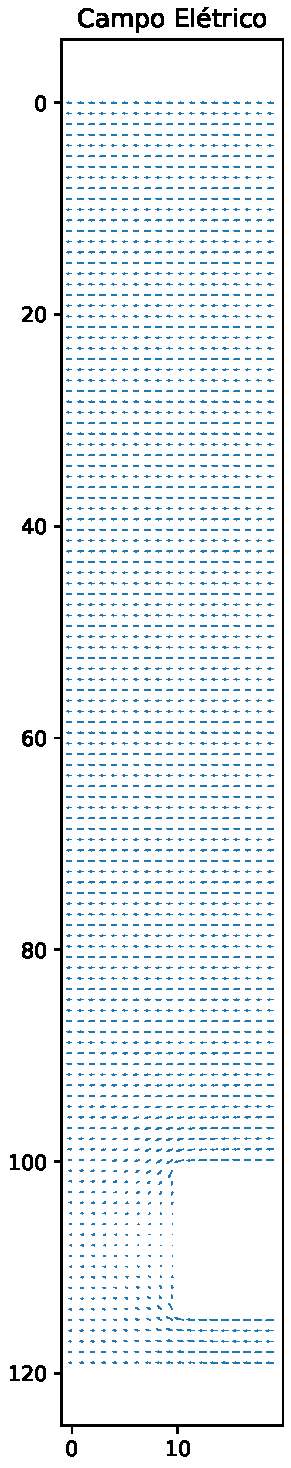
\includegraphics[height=210mm]{p2_campo_eletrico}
  \end{tabular}
  \caption{Linhas de campo para o Problema 1 (esquerda) e Problema 2 (direita). Esta é uma imagem vetorial (assim como as demais), é possível aumentar o zoom sem perder resolução.}
  \label{fig:campo}
\end{figure}


\newpage
\subsection{Resistência}

Anteriormente, foram usadas malhas de discretização de lado 1mm ou 2mm por motivos de vizualização. Agora, para calcular a resistência, foram usadas malhas de discretização de lado igual a 0.5mm ($k=2$) para ambos os problemas. As matrizes de potencial foram calculadas considerando um valor máximo de erro quadrático igual a $1 \times 10^{-10}$. Nessas condições, a convergência foi atingida após 55890 épocas para o Problema 1 e 2300 épocas para o Problema 2.


\subsubsection{Erros parciais}

As Figuras \ref{fig:erro_p1} e \ref{fig:erro_p2} mostram os valores dos erros quadráticos do potencial em função da época na escala log-log.

\begin{figure}[!ht]
  \centering
  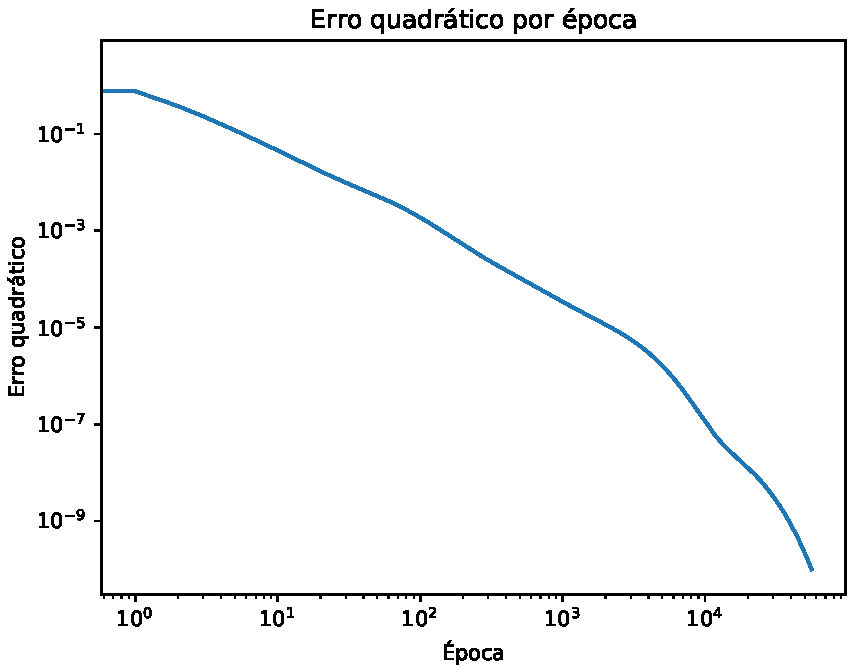
\includegraphics[width=0.63\textwidth]{p1_hist}
  \caption{Gráfico log-log do valor do erro quadrático em função da época para o Problema 1.}
  \label{fig:erro_p1}
\end{figure}

\begin{figure}[!ht]
  \centering
  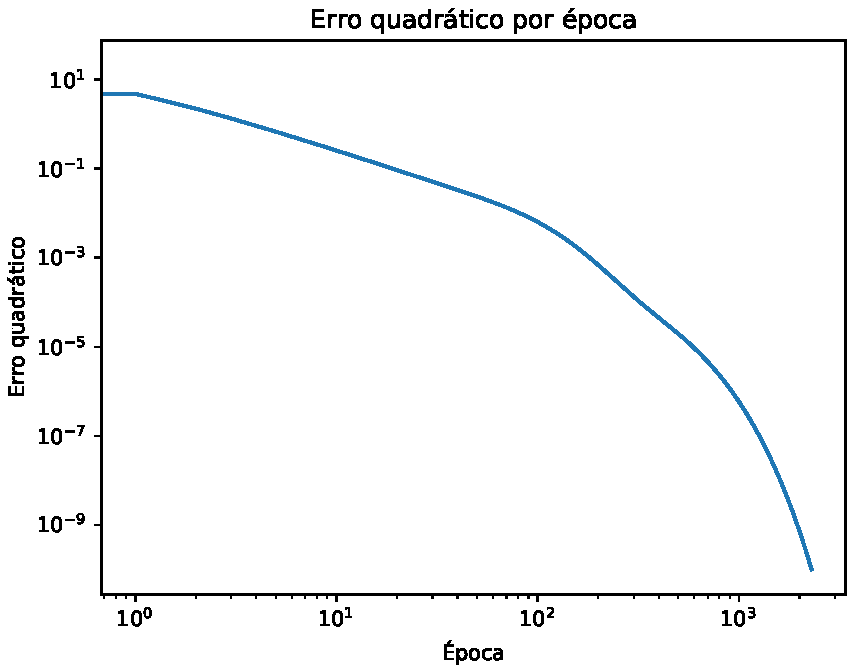
\includegraphics[width=0.63\textwidth]{p2_hist}
  \caption{Gráfico log-log do valor do erro quadrático em função da época para o Problema 2.}
  \label{fig:erro_p2}
\end{figure}


\subsubsection{Resistências parciais}

Esta análise foi feita para associar o valor de resistência calculada a partir de linhas em diferentes alturas na placa do Problema 1 (\texttt{template1}). Isso é mostrado na Figura \ref{fig:resist_table}, onde a linha azul indica o valor da resistência e a linha vermelha indica a mediana (considerando as resistências em todas as alturas). O eixo das abscissas indica a altura da placa considerada para o cálculo da resistência e o eixo das ordenadas indica o valor da resistência. Estes gráficos foram gerados a partir de um \texttt{template} com $k=2$, que representa uma malha de discretização de lado $h=1/k=0.5 mm$. Isto é, cada ponto do eixo das abscissas representa 0.5mm da altura real.

\bigskip

\begin{figure}[!ht]
  \begin{tabular}{cccc}
    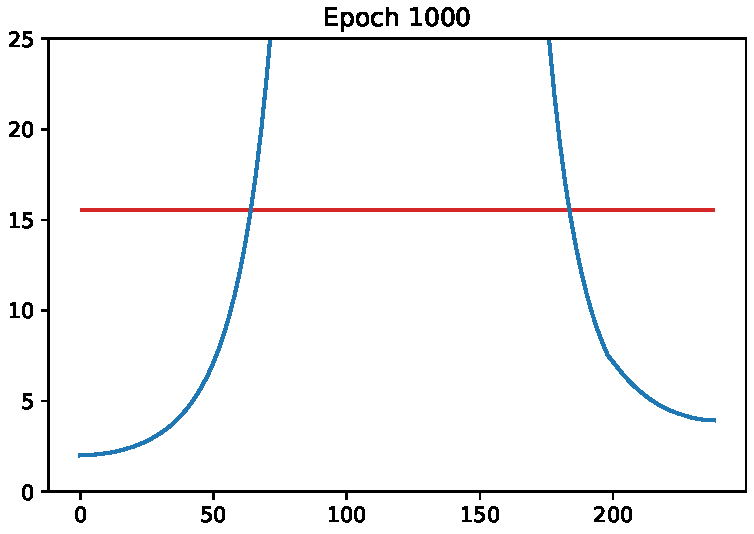
\includegraphics[width=0.22\linewidth]{res_1000}  &
    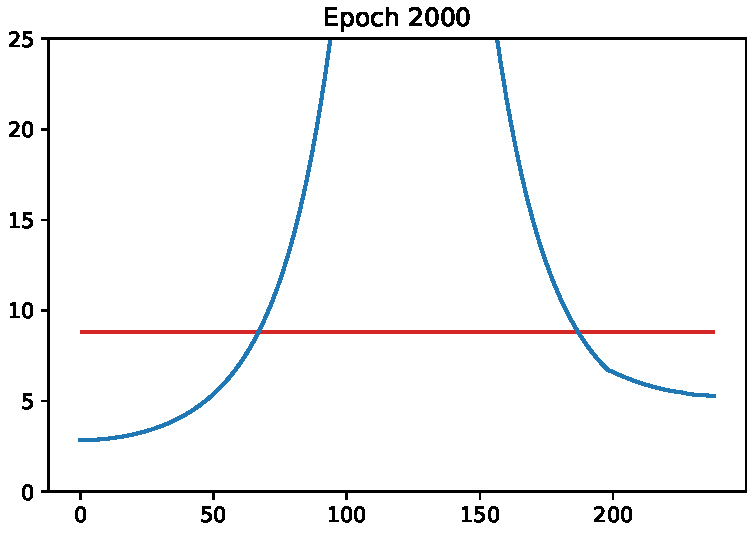
\includegraphics[width=0.22\linewidth]{res_2000}  &
    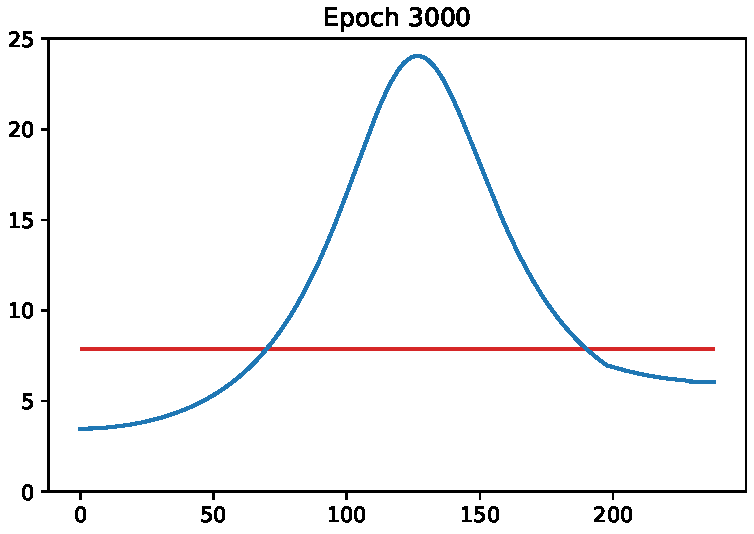
\includegraphics[width=0.22\linewidth]{res_3000}  &
    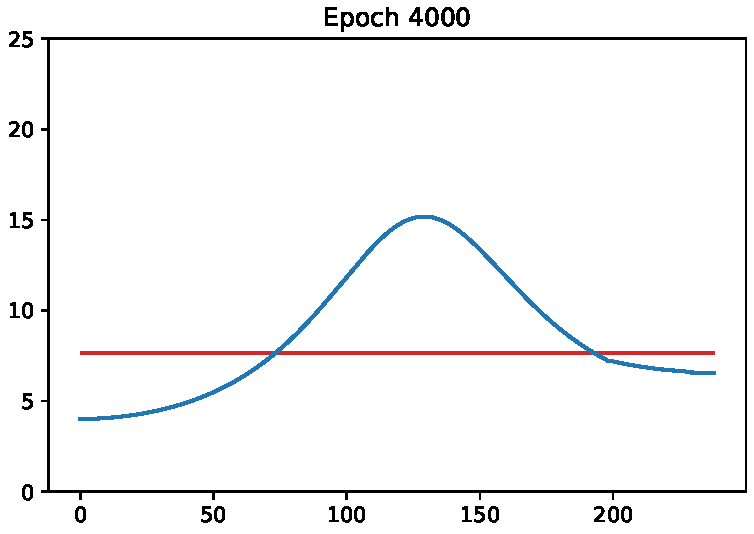
\includegraphics[width=0.22\linewidth]{res_4000}    \\

    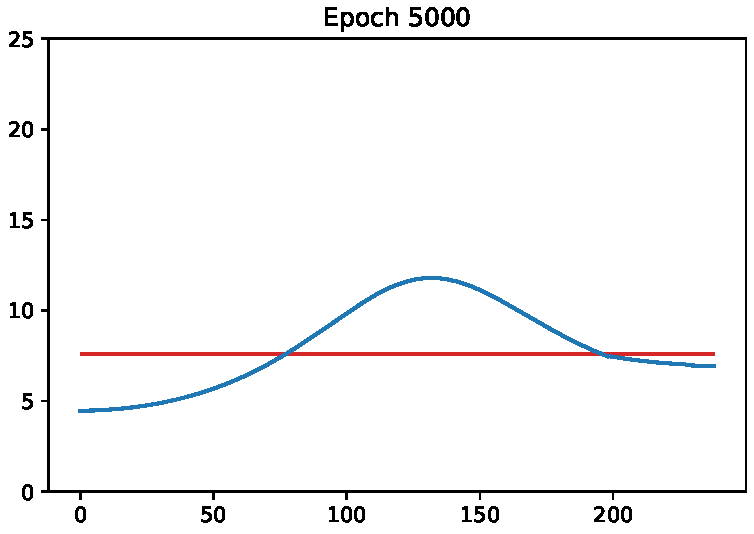
\includegraphics[width=0.22\linewidth]{res_5000}  &
    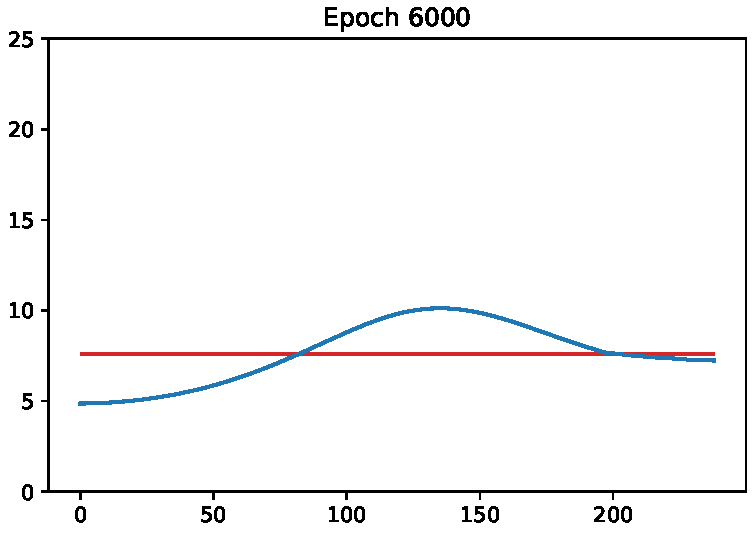
\includegraphics[width=0.22\linewidth]{res_6000}  &
    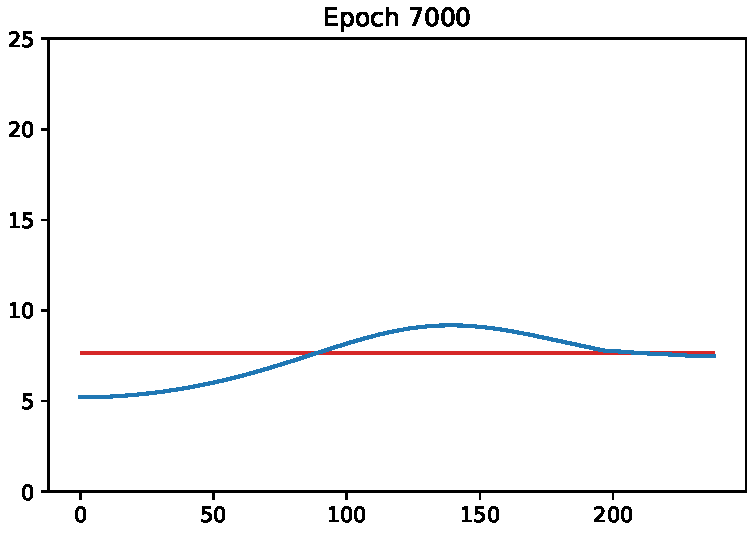
\includegraphics[width=0.22\linewidth]{res_7000}  &
    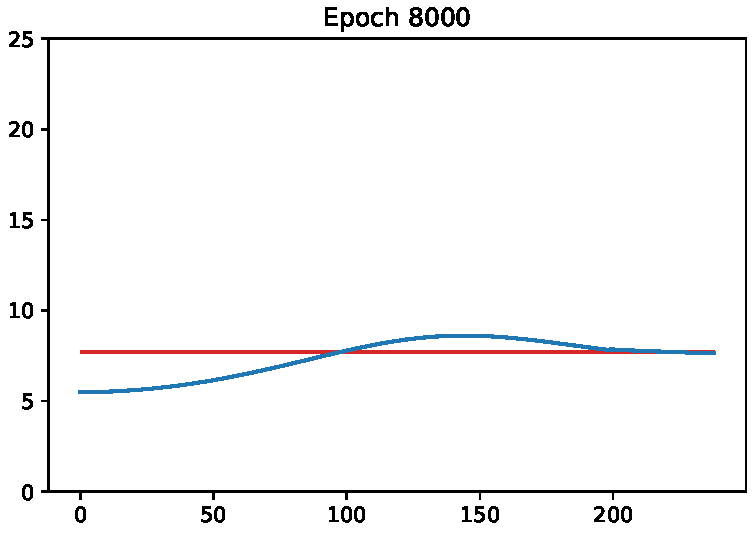
\includegraphics[width=0.22\linewidth]{res_8000}    \\

    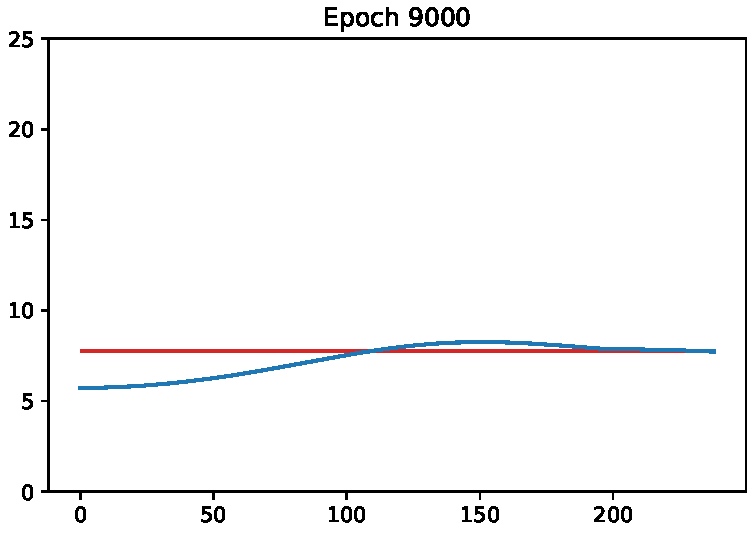
\includegraphics[width=0.22\linewidth]{res_9000}  &
    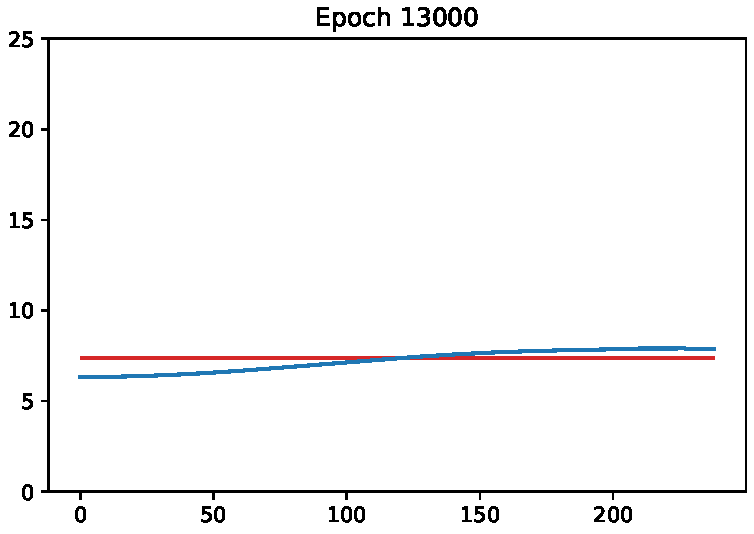
\includegraphics[width=0.22\linewidth]{res_13000} &
    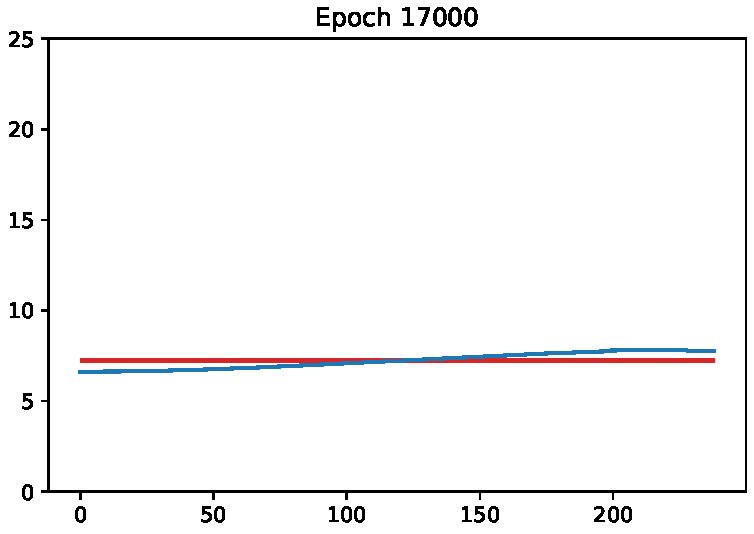
\includegraphics[width=0.22\linewidth]{res_17000} &
    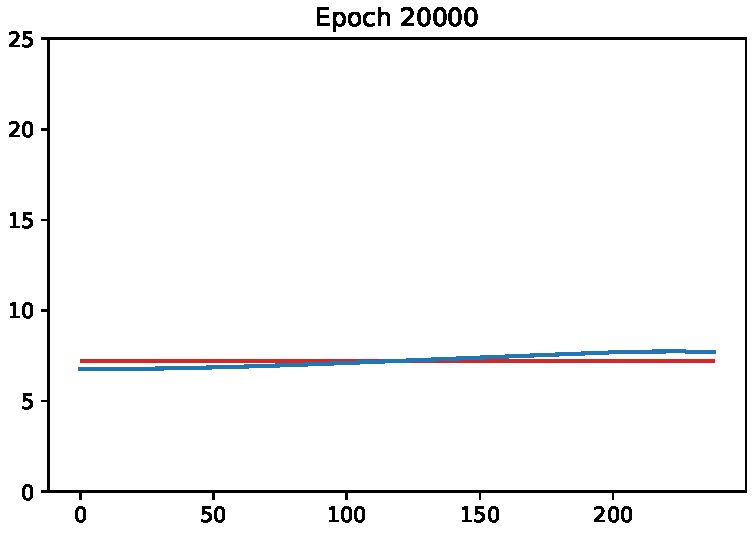
\includegraphics[width=0.22\linewidth]{res_20000}   \\

    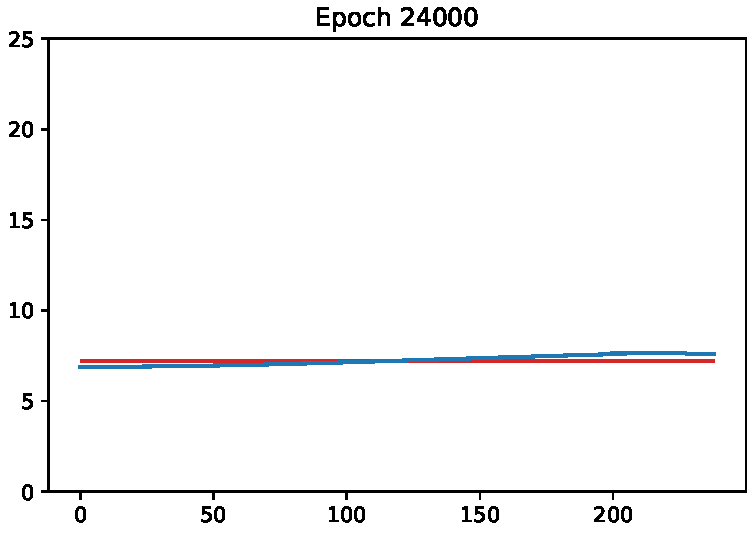
\includegraphics[width=0.22\linewidth]{res_24000} &
    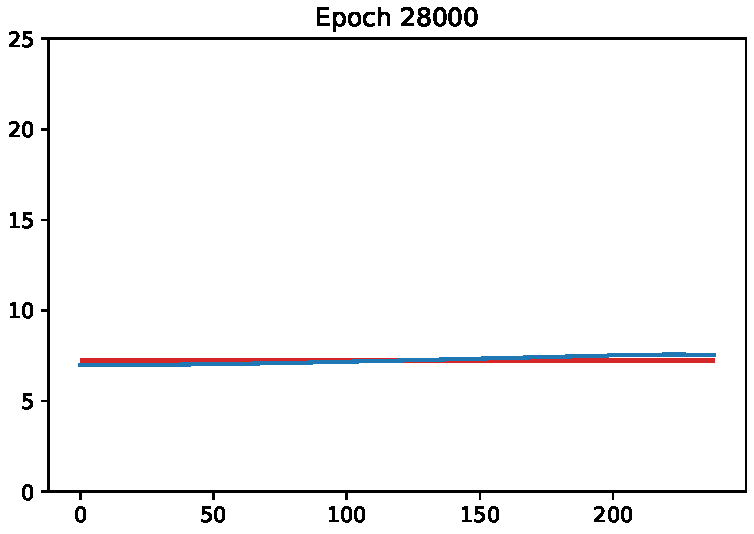
\includegraphics[width=0.22\linewidth]{res_28000} &
    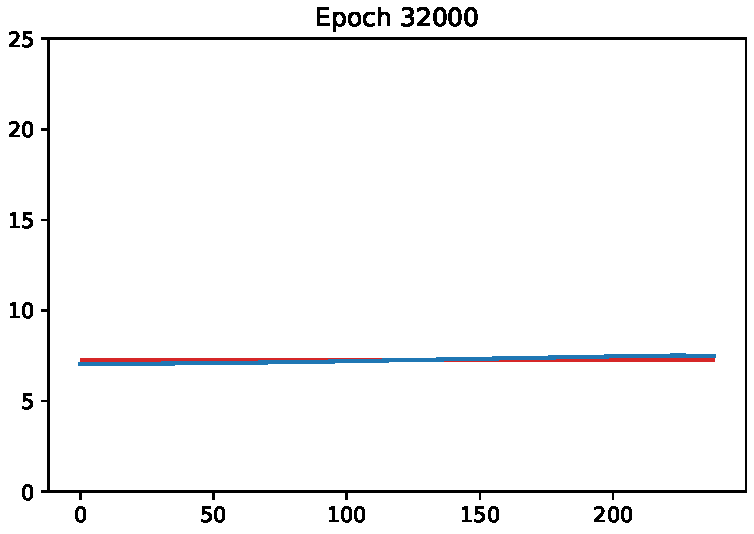
\includegraphics[width=0.22\linewidth]{res_32000} &
    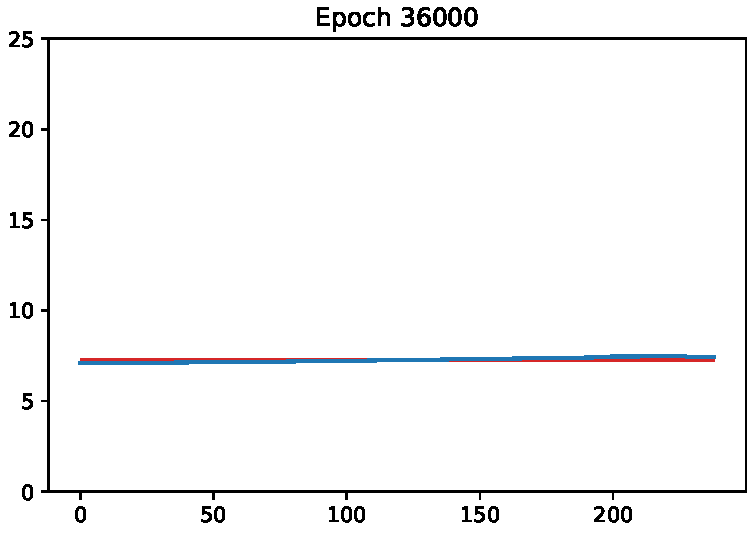
\includegraphics[width=0.22\linewidth]{res_36000}   \\

    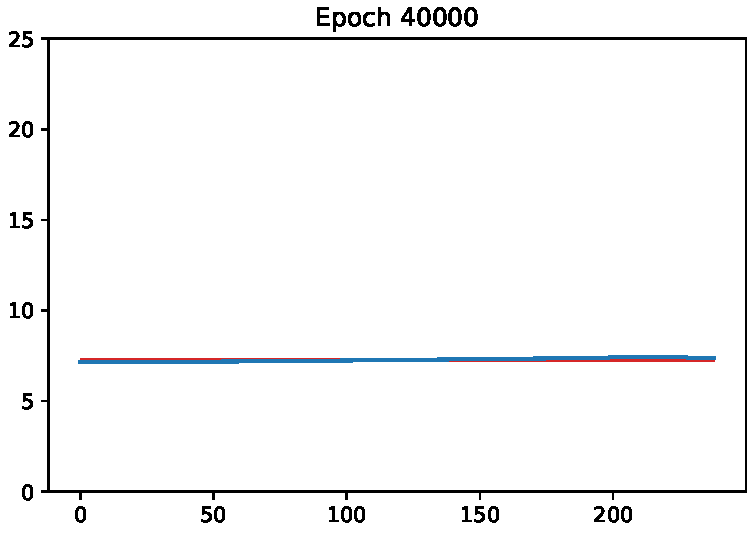
\includegraphics[width=0.22\linewidth]{res_40000} &
    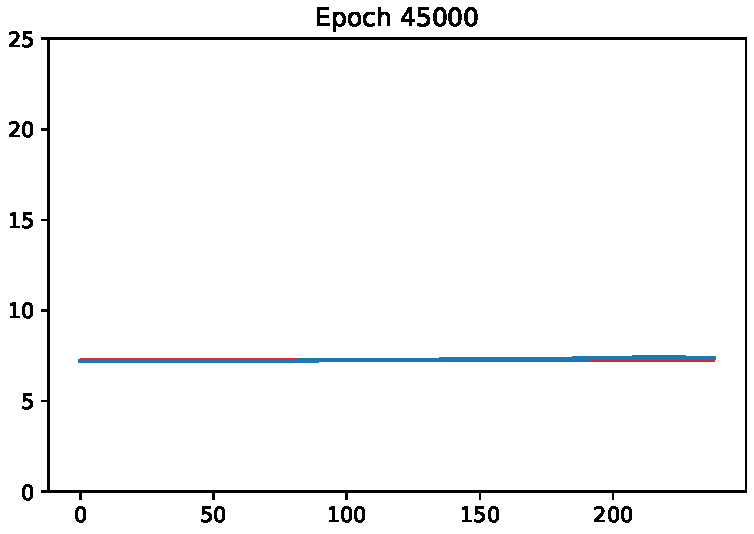
\includegraphics[width=0.22\linewidth]{res_45000} &
    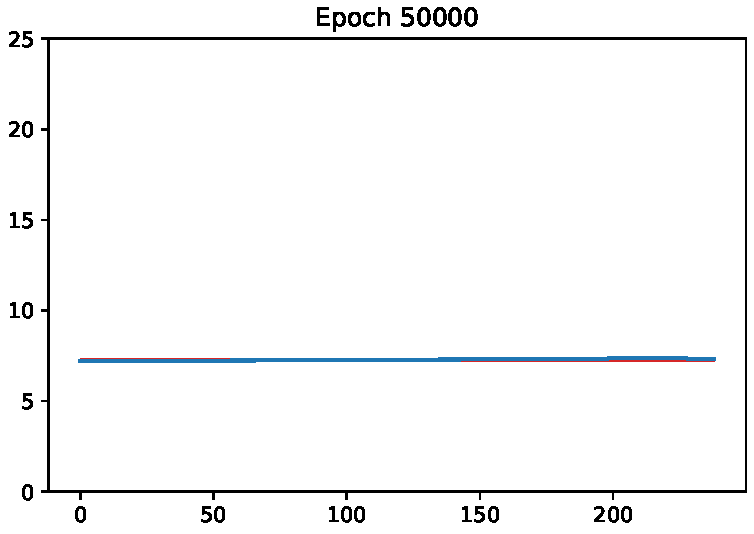
\includegraphics[width=0.22\linewidth]{res_50000} &
    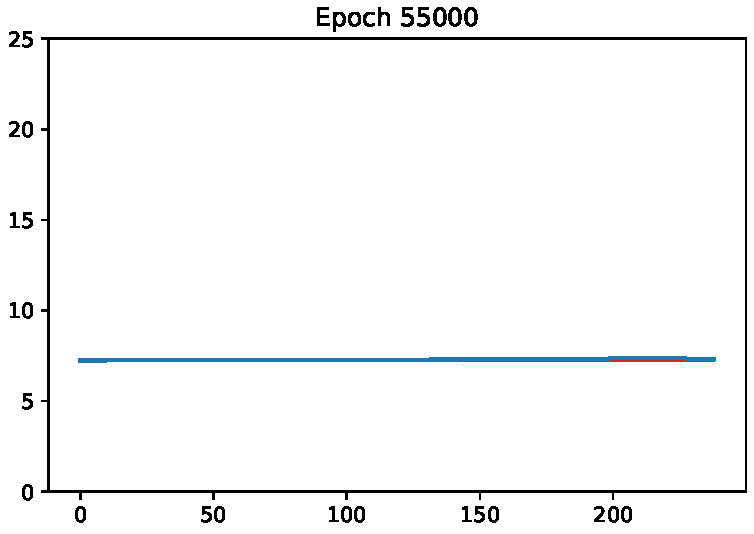
\includegraphics[width=0.22\linewidth]{res_55000}   \\
  \end{tabular}
  \caption{Valores de resistência para diferentes épocas (iterações)).}
  \label{fig:resist_table}
\end{figure}


\newpage
\subsubsection{Resistências finais}

As Figuras \ref{fig:res_p1} e \ref{fig:res_p2} mostram os valores de resistência calculados em função da altura (Problema 1) ou largura (Problema 2) da placa. As linhas vermelhas indicam a mediana considerando todas as medições de resistência e as linhas verdes indicam a mediana considerando apenas medições antes da região preenchida com vácuo ($y < k[b-(d+e)] = 200$ para o Problema 1 e $x < k[(a-c)/2] = 20$ para o Problema 2). Esta última será considerada como resposta final.

Assim, considerando o valor do estimador mediana amostral, chega-se à conclusão que o valor da resistência para o Problema 1 é $R \approx 7.28 \Omega$ e para o Problema 2 é $R \approx 0.36 \Omega$.

\begin{figure}[!ht]
  \centering
  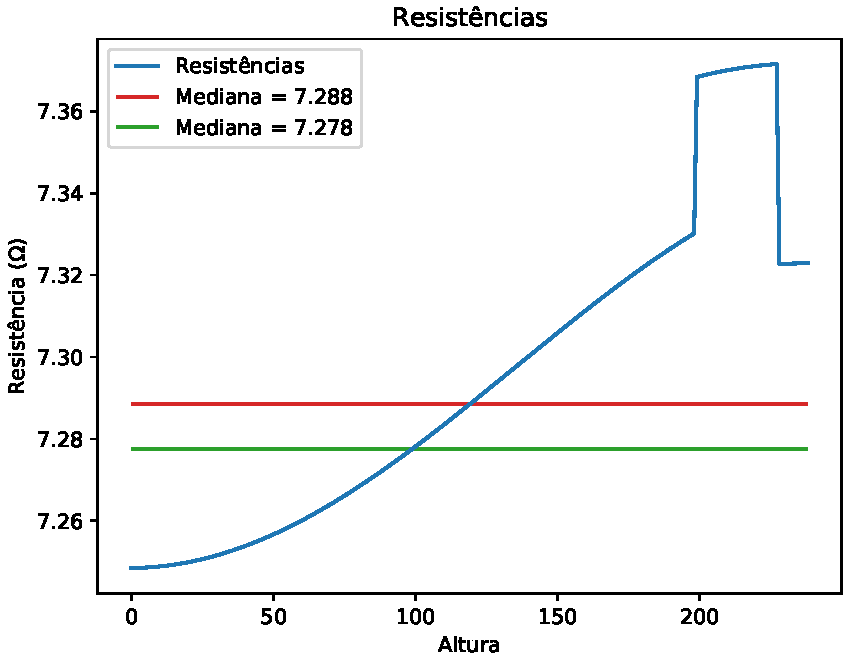
\includegraphics[width=0.7\linewidth]{p1_resistencias}
  \caption{Valores de resistência do Problema 1 em função da altura da placa na última época (55890).}
  \label{fig:res_p1}
\end{figure}

\begin{figure}[!ht]
  \centering
  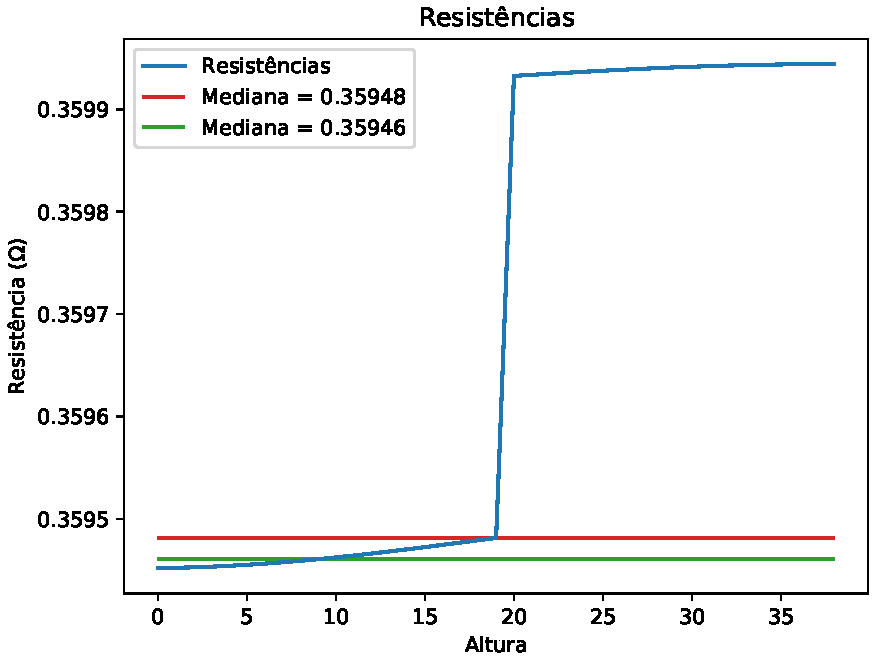
\includegraphics[width=0.7\linewidth]{p2_resistencias}
  \caption{Valores de resistência do Problema 2 em função da altura da placa na última época (2300).}
  \label{fig:res_p2}
\end{figure}


% \printbibliography

\end{document}
